\section{Resource management}

Effective resource management can be achieved through CPU multiplexing, process control, and efficient scheduling.

\subsection{CPU multiplexing}
CPU multiplexing enhances CPU utilization by allowing the processor to switch between different processes, such as when a program is waiting for input and other processes need to run. 
To minimize the overhead of context switching, it is crucial to optimize latency. 
This can be achieved by quantizing the time allocated to each process, ensuring efficient use of the CPU's capabilities.
\begin{figure}[H]
    \centering
    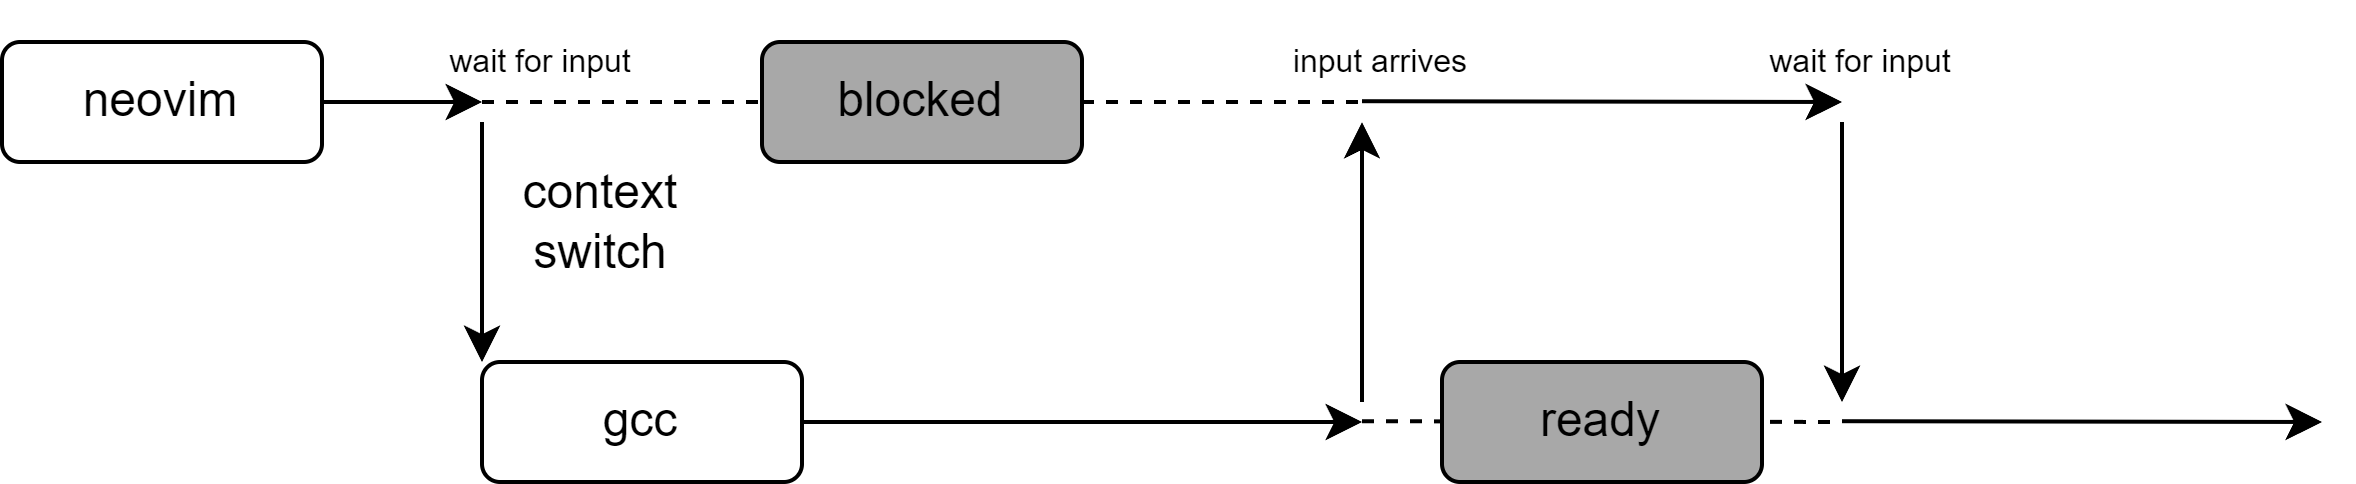
\includegraphics[width=0.75\linewidth]{images/mult.png}
    \caption{CPU multiplexing}
\end{figure}

\subsection{Process control}
The state of a process reflects its current condition and determines its capabilities, the resources it is using, and the conditions required to transition out of that state.
\begin{figure}[H]
    \centering
    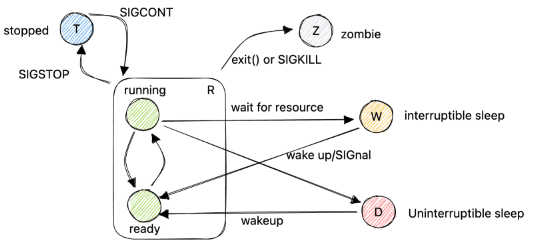
\includegraphics[width=0.75\linewidth]{images/proc.png}
    \caption{Process states}
\end{figure}
In Linux, each process is represented by a Process Control Block (PCB).
The PCB stores vital information about the process, including its Process Identifier (PID), process context (architectural state), virtual memory mappings, open files (including memory-mapped files), credentials (user/group ID), signal handling information, controlling terminal, priority, accounting statistics, and more.

In preemptive OS, process switching occurs when the kernel regains control, typically through mechanisms such as interrupts and exceptions. 
During a context switch, the current process's context is saved into its PCB, and the PCB of the next process is loaded into the machine's state, enabling seamless switching between processes.

\subsection{Scheduling}
The operating system uses several criteria to determine which process should run next, aiming to balance multiple objectives. 
Fairness is a key consideration, ensuring that no process is starved of resources. 
Throughput is also important, as the system seeks to maintain good overall performance. 
Efficiency is crucial as well, minimizing the overhead introduced by the scheduler itself. 
Additionally, the system must account for priority, reflecting the relative importance of different processes, and deadlines, where certain tasks must be completed within specific time constraints.

There is no single universal scheduling policy because these goals often conflict with one another, such as the tension between meeting deadlines and ensuring fairness. 
The appropriate solution varies depending on the problem domain, with General-Purpose OS (GPOSes) requiring different approaches than Real-Time OS (RTOSes): 
\begin{itemize}
    \item \textit{General-Purpose OS}: GPOSes prioritize fairness and throughput, although the specific definition of throughput can vary depending on the application. 
        These systems typically implement a CPU timeslice mechanism, where tasks are preempted based on their allocated timeslice, unless they are blocked. 
        Lower-priority tasks are allowed to consume their share of CPU resources, and the system is organized in a best-effort manner, meaning that while there are no guarantees, the OS strives to manage resources effectively.
    \item \textit{Real-Time OS}: RTOSes focus more on meeting deadlines and prioritizing tasks efficiently. 
        These systems assume that higher-priority threads do not always run continuously, but when a higher-priority thread becomes available, it is immediately granted control, without waiting for the current thread to complete its allocated processor time. 
        In cases where meeting deadlines is critical, the OS is classified as Hard Real-Time (Hard RT). 
        The emphasis in RTOS is on ensuring that high-priority tasks are executed promptly, reflecting their critical nature.
\end{itemize}
The main scheduling policies are the following. 
\begin{table}[H]
    \centering
    \begin{tabular}{|c|c|c|}
    \hline
    \textbf{Name} & \textbf{Goal}  & \textbf{Where it is used}    \\ \hline
    FIFO          & Turnaround     & Linux                        \\
    Round robin   & Response time  & Linux                        \\
    CFS           & CPU fair share & Linux                        \\
    EDF           & Real-time      & Linux                        \\
    MLFQ          & Response time  & Solaris, Windows, macOS, BSD \\
    SJF/SRTF/HRRN & Waiting time   & Custom                       \\ \hline
    \end{tabular}
\end{table}




